Many measurements of standard model properties or searches for new physics beyond the standard model performed within the CMS experiment rely on events with jets in the final state. Hence a good understanding of jet properties, like for instance the resolution of the jet transverse momentum is of major importance and a crucial ingredient for such kind of analyses. For example, many new physics searches are carried out based on jet final states. Here, QCD multijet events can fake the signature of possible new physics events and constitue a background process, since a mismeasurement of the jet momenta due to the limited detector resolution or the decay of heavy flavour quarks leads to a momentum imbalance in the event and consequently to measurable missing energy. The knowledge of the jet resolution is a hence keypoint in the prediction of such background contributions, as discussed in Chapter~\ref{chap:RA2}. \\
In this chapter, an analysis is presented where the jet-\pt resolution in data and in simulated events is derived. The method is based on momentum conservation in the transverse plane of dijet events and offers the possibility to cover a large phase space in \pt and $\eta$ with a sufficient statistical precision. A similar approach was already used in previous studies at $\sqrt{s}=7$\tev~\cite{1748-0221-6-11-P11002, thesis:Schroeder} while a complementary approach utilizes $\gamma +\rm{jet}$ events~\cite{CMS-AN-2010-141, CMS-AN-2011-004, CMS-AN-2013-179}. The measurement shown here is based on collision data corresponding to an integrated luminosity of $19.7$~\fbinv recorded at $\sqrt{s}=8$\tev in 2012.
\section{Basic Concept of the Dijet Asymmetry Method}
\label{sec:jer_method}
The measured jet transverse momentum is not necessarily equal to the energy of the original particle due to e.g. a limited detector resolution. This effect is quantified by the jet transverse momentum response R which is defined as 
\begin{equation}
  \mathrm{R} = \frac{\pt}{\pt^{\mathrm{particle}}} 
  \label{eq:response}
 \end{equation}
where \pt denotes the transverse momentum of the jet measured at detector level and $\pt^{\rm{particle}}$ is the transverse momentum of the original particle-level jet. The average response $\langle R \rangle$ is referred to as jet energy scale and calibrated such that $\langle R \rangle = 1$ for fixed $\pt^{\mathrm{particle}}$. The response usually depends on the jet momenta as well as on the pseudorapidity. This is expected since the quality of the jet measurement is directly related to the detector sub-components and the energy of the particles originating e.g. from the track-reconstruction efficiency or the individual amount of detector material. \\
\begin{figure}[!htp]
  \centering
  \begin{tabular}{c}
                \includegraphics[width=0.49\textwidth]{figures/TruthResponse_example_final_nominal_v4.pdf}
  \end{tabular}
  \caption{Jet response function for one example $|\eta_\mathrm{gen}|$ and $p_\mathrm{T, gen}$ interval derived from simulation.}
  \label{fig:response}
\end{figure}
In Fig.~\ref{fig:response} an example for a jet response distribution derived from simulation is shown where the transverse momentum of the particle-level jet is given by the \pt of the generated jet. Apparently the jet response consists generally of two components -- the gaussian-shaped core representing fluctuations around the mean and non-gaussian components refered to as tails. The core of the response is caused by the intrinsic resolution of the various sub-detector components and the precision of the jet clustering algorithms. The response tails are mainly caused by severe jet-mismeasurements. These can be e.g. detector effects like shower leakage or detector noise. On the other hand also physics processes contribute to the population of the response tails as e.g. semi-leptonic decays of heavy-flavour quarks contain neutrinos which obtain a certain amount of the momentum and leave the detector unnoticeable. \\
Finally, the relative jet transverse momentum resolution is defined as the width of the response distribution corresponding to the gaussian part and hence is a function of \pt and $\eta$ as well as the total response.\\
\\
One possibility to measure the resolution of the jet transverse momenta in data as well as in simulated events is to utilize the dijet asymmetry A. For events with at least two jets it is defined as
\begin{equation}
\label{eq:asymmdef}
  \mathrm{A} = \frac{p_{T,1} - p_{T,2}}{p_{T,1} + pt_{T,2}} \, .
 \end{equation}
 In this equation $p_{T,1}$ and $p_{T,2}$ correspond to the randomly ordered transverse momenta of the two leading jets. \\
 For a sufficient number of events the asymmetry is approximately normally distributed and its' standard deviation is given as
 \begin{equation}
 \label{eq:asymm_first}
  {\sigma_{\mathrm{A}}} = \left\lvert \frac{\partial A}{\partial p_{T,1}} \right\rvert \cdot \sigma(p_{T,1}) \oplus  \left\lvert \frac{\partial A}{\partial p_{T,2}} \right\rvert \cdot \sigma(p_{T,2})
 \end{equation}
 In an ideal dijet topology the two jets are exactly balanced at particle level. If they are in the same $\eta$ region, then $\langle p_{T,1} \rangle = \langle p_{T,2} \rangle = \langle \pt \rangle$ and $\sigma (p_{T,1}) = \sigma (p_{T,2}) = \sigma (\pt)$. This allows the simplification of Eq.~\ref{eq:asymm_first} and provides the following important relation between the width of the asymmetry $\sigma_{A}$ and the jet-\pt resolution $\sigma (p_{T})$
 \begin{equation}
 \label{eq:asymm}
  \frac{\sigma (p_{T})}{\langle p_{T} \rangle} = \sqrt{2} \cdot \sigma_{A}
 \end{equation}
Already at the Tevatron experiments~\cite{oai:arXiv.org:hep-ex/0012046, JetsD0}, the ATLAS experiment~\cite{Aad:2012ag} or in previous CMS analyses as stated above this relationship was utilized to measure the jet resolution from dijet events.  

\section{Apllication to Realistic Collision Events}
\label{sec:jer_application}
The measurement of the jet transverse momentum resolution in collision events is based on Eq.~\ref{eq:asymm}. As discussed in Section~\ref{sec:jer_method} the resolution is a function of \pt and $\eta$ so that the asymmetry distribution also has to be derived for different \pt and $\eta$ intervals. Since the relation between resolution and width of the asymmetry distribution is based on the assumption that the asymmetry is normally distributed only asymmetry distributions with at least 100 events are considered for the analysis. \\
\\
Beyond that the ideal dijet topology with exactly two jets being perfectly balanced is interfered with additional effects in realistic collision events. Very often further jet activity is occuring as momentum of the hard scattering process is transferred to soft-particles or jets arising from initial or final state radiation leading to momentum imbalance in the event. This additional jet activity can in good approximation be described by the variable $\alpha$ which is defined as
 \begin{equation}
\label{eq:alpha}
\alpha = \frac{p_{T,3}}{\pt^{ave}} \, .
\end{equation}
The presence of additional jets and the thereby introduced imbalance leads to a broadening of the observed asymmetry distribution. In order to determine the intrinsic resolution from such events the measured resolution has to be corrected for this bias. \\
Another reason for momentum differences between the particle-level and the detector-level jet leading to an overall momentum imbalance in an event is e.g. arising from out-of-cone showering effects in the jet-clustering procedure. This is an effect which requires a correction in the resolution measurement as well.\\
The application of corrections to the dijet asymmetry in practice is discussed in Section~\ref{sec:jer_corrections}.\\
\\
As the measurement of the resolution in collision data is based on the width of the dijet asymmetry distribution, a proper definition of the asymmetry width is of major importance.\\
From the tails of the detector response events with large asymmetries can emerge leading to non-gaussian tails in the asymmetry distributions. These shall not be considered in the calculation of the asymmetry width in order to not bias the determination of the asymmetry width one is interested in for the measurement of the resolution. Hence the asymmetry width has to be defined such that the central part of the distribution is approximated reasonably well by a gaussian distribution. 
\begin{figure}[!tp]   
  \centering
  \begin{tabular}{cc}
                \includegraphics[width=0.49\textwidth]{figures/AsymmHistosDataWithRatio_Eta0_pt5_alpha2_final_nominal_NoTruncation_v4.pdf} &
                \includegraphics[width=0.49\textwidth]{figures/AsymmHistosSimWithRatio_Eta0_pt5_alpha2_final_nominal_NoTruncation_v4.pdf} \\ 
                \includegraphics[width=0.49\textwidth]{figures/AsymmHistosDataWithRatio_Eta0_pt5_alpha2_final_nominal_v4.pdf} &
                \includegraphics[width=0.49\textwidth]{figures/AsymmHistosSimWithRatio_Eta0_pt5_alpha2_final_nominal_v4.pdf} \\
                \includegraphics[width=0.49\textwidth]{figures/AsymmHistosDataWithRatio_Eta0_pt5_alpha2_final_nominal_95Truncation_v4.pdf} &
                \includegraphics[width=0.49\textwidth]{figures/AsymmHistosSimWithRatio_Eta0_pt5_alpha2_final_nominal_95Truncation_v4.pdf} \\
  \end{tabular}
  \caption{Asymmetry distributions for data (left) and simulation (right) compared to gaussian distributions obtained with standard deviations corresponding to 0\% truncation (top), 1.5\% truncation (middle) and 5\% truncation (bottom) of the tail regions.}
  \label{fig:asymm_width}
\end{figure}
In Fig.~\ref{fig:asymm_width} the asymmetry distribution in data and in simulation for a certain $|\eta|$, $\pt^{ave}$ and $\alpha$ interval is compared to gaussian distributions where the standard deviation of the gaussian function is chosen such that it corresponds to different asymmetry widths. The width of the asymmetry is determined by taking the whole distribution into account or by truncating a certain percentage in the tail regions. It is visible that the core part of the asymmetry distribution can in good approximation be described by a gaussian function if the tails are neglected in the calculation of the asymmetry width as long as the truncation is not rejecting parts of the gaussian core.\\
Thus the asymmetry width is in this analysis calculated as $98.5\%$-truncated root-mean-square
\begin{equation}
 \sigma_A = \mathrm{RMS}_{98.5\%} = \sqrt{\frac{1}{\sum_{i} y_i} \sum_{i} y_i \cdot A_i^2}  
\end{equation} 
where $y_i$ denotes the frequency of the asymmetry value $A_i$ and the sum over i includes all values such that $98.5\%$ of the total asymmetry distribution are covered. The statistical uncertainty is given by
\begin{equation}
\Delta \sigma_A = \Delta \mathrm{RMS}_{98.5\%} = \frac{\mathrm{RMS}_{98.5\%}}{\sqrt{\, 2 \cdot \mathrm{n_\mathrm{eff}}}} \,
\end{equation} 
with the number of effective entries $n_\mathrm{eff}$ in the specified interval for which the asymmetry distribution has been derived. 

\section{Samples and Event Selection}
\label{sec:jer_selection}
In this section the data samples used for the analysis are specified (Section~\ref{subsec:jer_samples_and_trigger}). Furthermore, selection criteria applied on data and simulated events in order to select events with a dijet-like topology are discussed (Section~\ref{subsec:jer_sel_cuts}). 

\subsection{Datasets and Triggers}
\label{subsec:jer_samples_and_trigger}
In this analysis, multijet events from pp collisions are considered which have been recorded in 2012 with the CMS detector at $\sqrt{s}=8$\tev. The following collision data samples are used \\
\\
$\verb+/Jet/Run2012A-22Jan2013-v1/AOD+$ \\ 
$\verb+/JetHT/Run2012B-22Jan2013-v1/AOD+$ \\
$\verb+/JetMon/Run2012B-22Jan2013-v1/AOD+$ \\
$\verb+/JetHT/Run2012C-22Jan2013-v1/AOD+$ \\
$\verb+/JetMon/Run2012C-22Jan2013-v1/AOD+$ \\
$\verb+/JetHT/Run2012D-22Jan2013-v1/AOD+$ \\
$\verb+/JetMon/Run2012D-22Jan2013-v1/AOD+$. \\
\\
From these samples only luminosity sections fulfilling certain data quality criteria are considered in the analysis \footnote{Luminosity sections which are taken into account for the analysis are listed in the Golden JSON file $Cert\_190456-208686\_8TeV\_22Jan2013ReReco\_Collisions12\_JSON.txt$ }. The collected data sample corresponds to an integrated luminosity of $19.7$~\fbinv. \\
\\
Multijet events are pre-selected by a set of triggers based on the average transverse momentum $\pt^{ave}$ of the two leading jets in the event:  
\begin{equation}
 p_{T}^{ave} = \frac{1}{2} (p_{T,1} + p_{T,2}).
\end{equation} 
Different trigger paths are combined which feature a good coverage of the $\pt^{ave}$ spectrum since they have different minimum $\pt^{ave}$ thresholds. In Tab.~\ref{tab:trigger} the different trigger paths used for this analysis are summarized together with the $\pt^{ave}$ value for which the respective trigger reaches the $99\%$ efficiency plateau (taken from~\cite{website:HamburgCalib}).

\begin{table}[!tp]
\centering
\caption{Trigger paths with $\pt^{ave}$ thresholds at which the trigger efficiency reaches the $99\%$ efficiency plateau. The thresholds are given for PFCHS jets.}
\label{tab:trigger}
% \makebox[\linewidth]{
\begin{tabular}{clccc}
%\multicolumn{6}{c}{} \\
%\hline
 & & & & \\
 & Trigger & & $\pt^{ave}$ threshold [GeV] & \\
 & & & & \\
\hline
 & & & & \\
 & $\mathrm{HltDiPFJetAve40}$ & & 62 & \\
 & & & & \\
 & $\mathrm{HltDiPFJetAve80}$ & & 107 & \\
 & & & & \\
 & $\mathrm{HltDiPFJetAve140}$ & & 175 & \\
 & & & & \\
 & $\mathrm{HltDiPFJetAve200}$ & & 242 & \\
 & & & & \\
 & $\mathrm{HltDiPFJetAve260}$ & & 310 & \\
 & & & & \\
 & $\mathrm{HltDiPFJetAve320}$ & & 379 & \\
 & & & & \\
 & $\mathrm{HltDiPFJetAve400}$ & & 467 & \\
 & & & & \\
\hline
\end{tabular}%}
\end{table} 
Simulated events are from the sample $/QCD_Pt-15to3000_TuneZ2_Flat_8TeV_pythia6$ created in the series $/Summer12_DR53X-PU_S10_START53_V7A-v1/AODSIM$. They are generated with the \pythia event generator and the full detector simulation. The simulated events are weighted depending on their $\hat{\pt}$ in order to regain a physical multijet spectrum.  

\subsection{Selection Criteria}
\label{subsec:jer_sel_cuts}
The physics objects used in the analysis are reconstructed with the particle-flow algorithm~\cite{CMS-PAS-PFT-09-001}. In order to reduce a possible impact from pileup, charged hadrons associated with a pileup vertex are removed from the event. This is referred to as charged-hadron subtraction (CHS). All jets -- in data as well as in simulation -- are clustered with the anti-$k_T$ algorithm using a distance parameter of $R=0.5$. In addition, jets are calibrated by applying jet energy corrections containing residual corrections for data. The event reconstruction is done using the CMSSW framework series $\rm{CMSSW\_5\_3\_X}$ with the global tag $\rm{FT\_53\_V21\_AN6}$ for data and $\rm{START53\_V27}$ for simulation. \\
\\
The two leading jets in each event have to fulfill loose jet identification criteria \todo{Jet ID}. If there is a third jet in the event, it has to fulfill this requirement as well. In the analysis a minimum \pt threshold of 10\gev is introduced for the first three leading jets. If an event has no third jet with \pt above 10\gev, the event is rejected in order to mitigate effects from pile-up. \\
\\
In order to enrich the sample with events close to the ideal dijet topology with two jets pointing into opposite directions in the transverse plane and to reject events with very large asymmetries the two leading jets have to fulfill 
\begin{equation}
|\Delta \phi| > 2.7 \; \mathrm{with} \; \Delta \phi = \Delta \phi(\vec{p_{T,1}}, \vec{p_{T,2}}) \, .
\end{equation}
As the resolution is a function of the transverse momentum and $|\eta|$ the asymmetry is calculated in various intervals of $|\eta|$ and $\pt^{ave}$ which are summarized in Tab.~\ref{tab:binning}. The $\pt^{ave}$ intervals are chosen such that the interval boundaries correspond to the offline $\pt^{ave}$-thresholds of the various different triggers. This ensures that the intervals belong to only one trigger. If a trigger provides enough statistical precision, the interval is separated into two. \\
The $|\eta|$ intervals are chosen such that they correspond to different sub-detector components, if possible. In the forward region of the detector, mainly jets with low transverse momentum are expected corresponding to triggers with low $\pt^{ave}$ thresholds. Since these are highly prescaled only few events populate the high $|\eta|$ region and prohibit a finer $\eta$-binning there. \\
\begin{table}[!tp]
\centering
\caption{Overview of the $|\eta|$ and $\pt^{ave}$ interval boundaries used for the resolution measurement.}
\label{tab:binning}
% \makebox[\linewidth]{
\begin{tabular}{ccc}
%\multicolumn{5}{c}{} \\
\hline
 & &  \\
 $|\eta|$ & & $\pt^{ave}$ [GeV] \\
 & &  \\
\hline
 & &  \\
 0.0, 0.5, 1.1, 1.7, 2.3, 2.8, 3.2, 5.0 & & 62, 107, 175, 205, 242, 270, 310, 335, 379, 410, 467, 600, 1000, $\infty$ \\
 & &  \\
\hline
\end{tabular}%}
\end{table} 
\\
As discussed in Section~\ref{sec:jer_application} events with a topology of exactly two high-\pt jets and no further jet activity are almost not existent in realistic collisions. To select a sample which offers many events that maintain a dijet-like structure, a maximum $\alpha$ threshold of $\alpha_\mathrm{max} = 0.25$ is introduced. \\
In order to account for the $\alpha$ dependence of the measured asymmetry distributions the $\pt^{ave}$ and $|\eta|$ intervals for the resolution measurement are further subdivided in various $\alpha$ intervals. The upper boundaries of the $\alpha_\mathrm{max}$ intervals are $0.1, 0.125, 0.15, 0.175, 0.2, 0.225, 0.25$. Each interval ranges from $\alpha = 0.0$ to the respective upper boundary. \\
\\
For the simulated sample two further things have to be considered related to the modelling of pileup. The first problem is that sometimes the $\hat{\pt}$ of an additional pileup event is larger than the $\hat{\pt}$ of the hard interaction resulting in events with extremely large weights. In order to protect the sample against such cases simulated events are rejected, if the \pt of one of the two leading jets is larger than $2 \cdot \hat{\pt}$.\\
The second issue is that the QCD sample is generated with a certain estimated pileup scenario. This is not necessarily the same as the observed pileup distribution in data. Therefore the simulated events are reweighted to match the pileup conditions in data. The pileup distribution in data is different for each individual trigger. This is due to the fact that the pileup conditions changed within the running periods in 2012 and due to the different prescales of the individual triggers which also changed over time each trigger path has an individual observed pileup distribution. Therefore each simulated event is reweighted to match the pileup scenario in the data distribution of that particular trigger path to which the simulated event would belong depending on the $\pt^{ave}$ of the event. This procedure can be checked by comparing the distribution of the number of primary vertices in data and simulation before and after reweighting since the number of primary vertices is a measure for the pileup activity in an event. The result is shown in Fig.~\ref{fig:pu_reweight} for the trigger path with the highest $\pt^{ave}$ threshold used in the analysis and shows a good agreement especially in the bulk of the distribution. The distributions of primary vertices before and after reweighting the pileup scenario of the other trigger paths relevant for the analysis are shown in Appendix \todo{app:pu reweight}. The pileup weight is considered as a multiplicative factor for each simulated event.
\begin{figure}[!tp]
  \centering
  \begin{tabular}{cc}
                \includegraphics[width=0.49\textwidth]{figures/NVtx_HltDiPFJetAve400_AfterTriggerSelection.pdf} &
                \includegraphics[width=0.49\textwidth]{figures/NVtx_HltDiPFJetAve400_AfterPUReweighting.pdf}
  \end{tabular}
  \caption{Distribution of number of primary vertices in data and simulation before (left) and after (right) reweighting of the pileup scenario in simulation for trigger path HltDiPFJetAve400.}
  \label{fig:pu_reweight}
\end{figure}

The resulting inclusive $\pt^{ave}$ spectrum of events after the described selection in data and in simulation as well as the \pt spectra of the first three leading jets are shown in Fig.~\ref{fig:ptave_spec}. The number of simulated events in each trigger $\pt^{ave}$ interval is normalized to the respective integral in data. 
\begin{figure}[!tp]
  \centering
  \begin{tabular}{cc}
                \includegraphics[width=0.49\textwidth]{figures/PtAve__AfterAsymmHistos.pdf} &
                \includegraphics[width=0.49\textwidth]{figures/Jet1Pt__AfterAsymmHistos.pdf} \\
                \includegraphics[width=0.49\textwidth]{figures/Jet2Pt__AfterAsymmHistos.pdf} &
                \includegraphics[width=0.49\textwidth]{figures/Jet3Pt__AfterAsymmHistos.pdf}

  \end{tabular}
  \caption{Inclusive $\pt^{ave}$ spectrum of events after the total selection in data and in simulation (top left), leading jet-\pt (top right), subleading jet-\pt (bottom left) and third jet-\pt (bottom right).}
  \label{fig:ptave_spec}
\end{figure}

Finally, some exemplary asymmetry distributions obtained after the dedicated selection described here are depicted in Fig.~\ref{fig:asymm_dists} for data and simulated events. 
\begin{figure}[!tp]
  \centering
  \begin{tabular}{cc}
                \includegraphics[width=0.49\textwidth]{figures/AsymmHistos_Eta0_pt4_alpha1_final_nominal_v4.pdf} &
                \includegraphics[width=0.49\textwidth]{figures/AsymmHistos_Eta0_pt9_alpha1_final_nominal_v4.pdf} \\ 
                \includegraphics[width=0.49\textwidth]{figures/AsymmHistos_Eta0_pt4_alpha5_final_nominal_v4.pdf} &
                \includegraphics[width=0.49\textwidth]{figures/AsymmHistos_Eta0_pt9_alpha5_final_nominal_v4.pdf}
  \end{tabular}
  \caption{Some example asymmetry distributions for the lowest $|\eta|$ region, two medium $\pt^{ave}$ intervals and for a low (top row) and a high (bottom row) $\alpha$ interval.}
  \label{fig:asymm_dists}
\end{figure}

\section{Corrections to the Dijet Asymmetry}
\label{sec:jer_corrections}
The fundamental relation between the width of the asymmetry distribution and the jet energy resolution as expressed in Eq.~\ref{eq:asymm} holds in this form only for the case of an ideal dijet topology. In real collision events various effects can occur that disturb the exact balance of the two jets. Such effects can be soft radiation or additional jets originating from the hard scattering. They lead to imbalance in the event and hence broaden the oberserved asymmetry distribution resultng in an increased measured resolution. In order to determine the intrinsic resolution, the measured one has to be corrected for such effects. These corrections are explained in the following Sections~\ref{subsec:jer_corrections_alpha} and ~\ref{subsec:jer_corrections_pli}.

\subsection{Correction for Additional Jet Activity}
\label{subsec:jer_corrections_alpha}
In addition to the two jets originating from the hard interaction further jets can occur in an event from the emission of additional partons or pileup. The additional jet activity in the event is quantified by $\alpha$ introduced in Eq.~\ref{eq:alpha} which is the fractional \pt of the third jet. The impact from jets beyond the third one is neglected since there impact is expected to be small due to the strongly decreasing jet-production cross-section. \\
\\
The imbalance contribution arising from additional jet activity is taken care of by an extrapolation procedure. As described in Section~\ref{subsec:jer_sel_cuts} the asymmetry distribution is calculated for several intervals in $|\eta|$ and $\pt^{ave}$ with different selections on the maximum value of $\alpha$ ($=\alpha_{max}$). For each of these individual selections the width of the asymmetry is determined as stated in Section~\ref{sec:jer_application}. The measured values of $\sigma_{A}(\alpha_{max})$ are extrapolated to $\alpha_{max} \rightarrow 0$ assuming a linear behaviour. The y-intercept of the fitted linear function represents the resolution without further jet activity in the event while the statistical uncertainty is given by the respective fit error. The extrapolation procedure for two exemplary $|\eta|$ and $\pt^{ave}$ intervals is illustrated in Fig.~\ref{fig:extrapol} (further extrapolations are shown in Appendix \todo{appendix: extrapol}). \\
\\
\begin{figure}[!tp]
  \centering
  \begin{tabular}{cc}
                \includegraphics[width=0.49\textwidth]{figures/Extrapol_Eta0_pt4_final_nominal_v4.pdf} &
                \includegraphics[width=0.49\textwidth]{figures/Extrapol_Eta0_pt9_final_nominal_v4.pdf}
  \end{tabular}
  \caption{Two examplary extrapolations of measured values for $\sigma_\mathrm{A}$ in data and simulation to obtain the result at zero additional jet activity.}
  \label{fig:extrapol}
\end{figure}
As stated in Section~\ref{subsec:jer_sel_cuts} the selection is performed in inclusive intervals of $\alpha < \alpha_{max}$. This results in a correlation of the measured values of $\sigma_\mathrm{A}$ for a particular $\pt^{ave}$ interval. In order to obtain a realistic estimate of the statistical uncertainty the correlation is propagated to the extrapolation fit. \\
In some more detail this means that the measured data points shall be described by a linear function $y=a \cdot x+b$. Thus the parameters a and b have to be determined for known $x$, $y$ and covariance matrix $C$ by minimizing the following $\chi^2$ 
\begin{equation}
dy^T \cdot C^{-1} \cdot dy
\end{equation}
where $dy = y_{\mathrm{measured}} - y_{\mathrm{predicted}}$. In this analysis the following relations apply $y=\sigma_\mathrm{A}(\alpha_{max})$, $x=\alpha_{max}$ and $b=\sigma_\mathrm{A}(\alpha_{max} \rightarrow 0)$. \\
Under the assumption that all events that belong to $\alpha$ interval $i$ are also completely included in the next higher $\alpha$ interval $j$~\footnote{This assumption is only almost true since the asymmetry distributions are truncated to reject non-gaussian components.} the covariance matrix is given by
\begin{equation}
C_{i,j}(\sigma_{A_i},\sigma_{A_j}) = (\Delta \sigma_{A_i})^2 \, \frac{\sigma_{A_i}}{\sigma_{A_j}} \, (\frac{n_i}{n_j})^2 
\end{equation}
where $n$ is the number of events in that particular interval. The function minimization itself is performed with the Minuit package~\cite{Minuit}. 

\begin{figure}[!htp]
  \centering
  \begin{tabular}{cc}
                \includegraphics[width=0.49\textwidth]{figures/GoodnessOfFit_Eta0_final_nominal_v4.pdf} &
                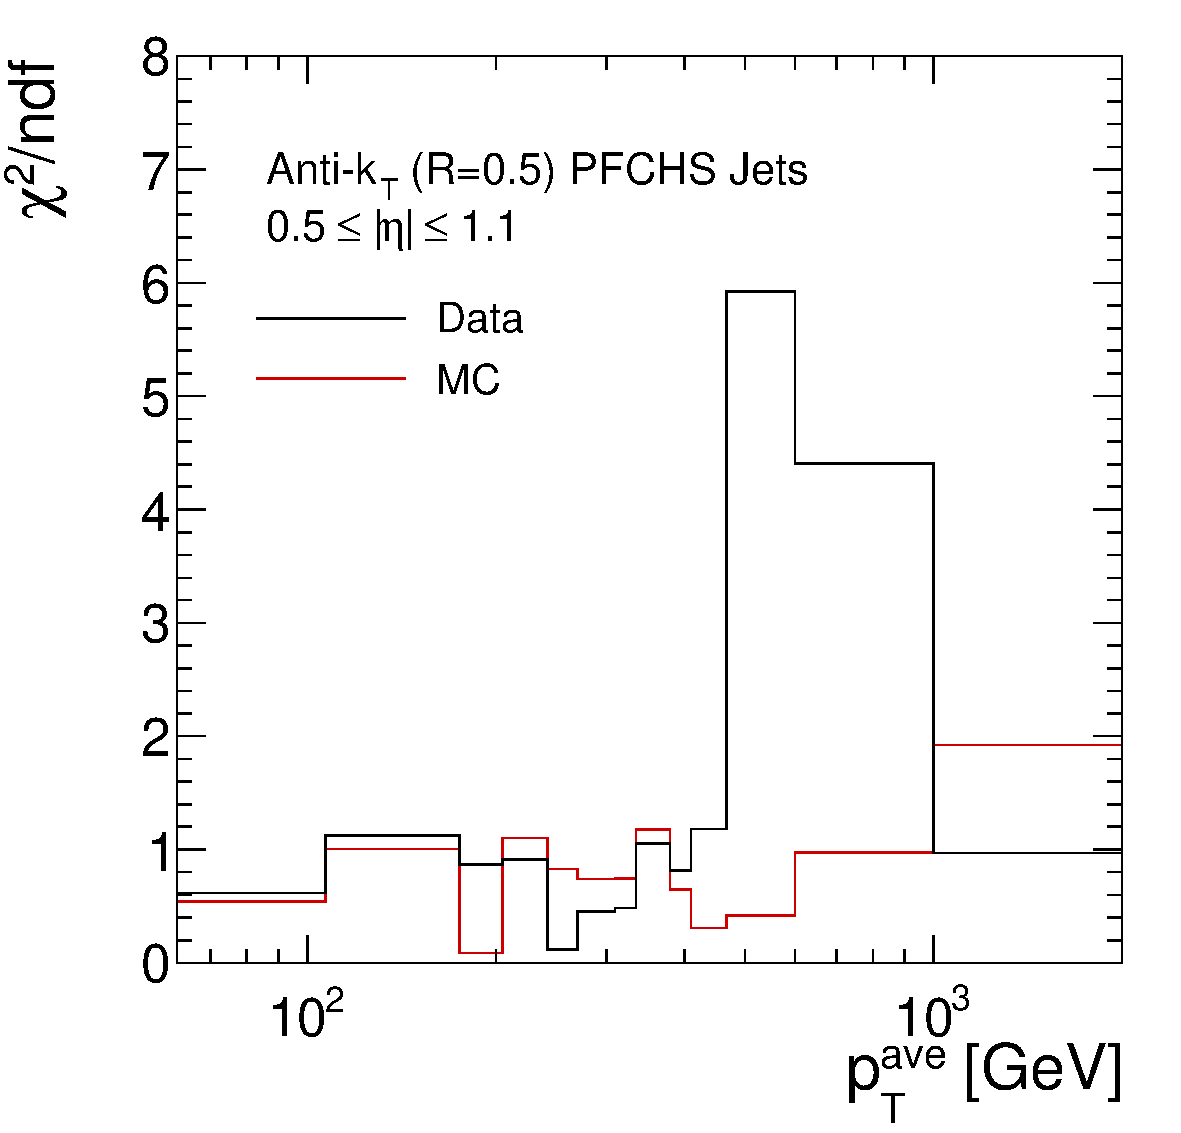
\includegraphics[width=0.49\textwidth]{figures/GoodnessOfFit_Eta1_final_nominal_v4.pdf} \\
                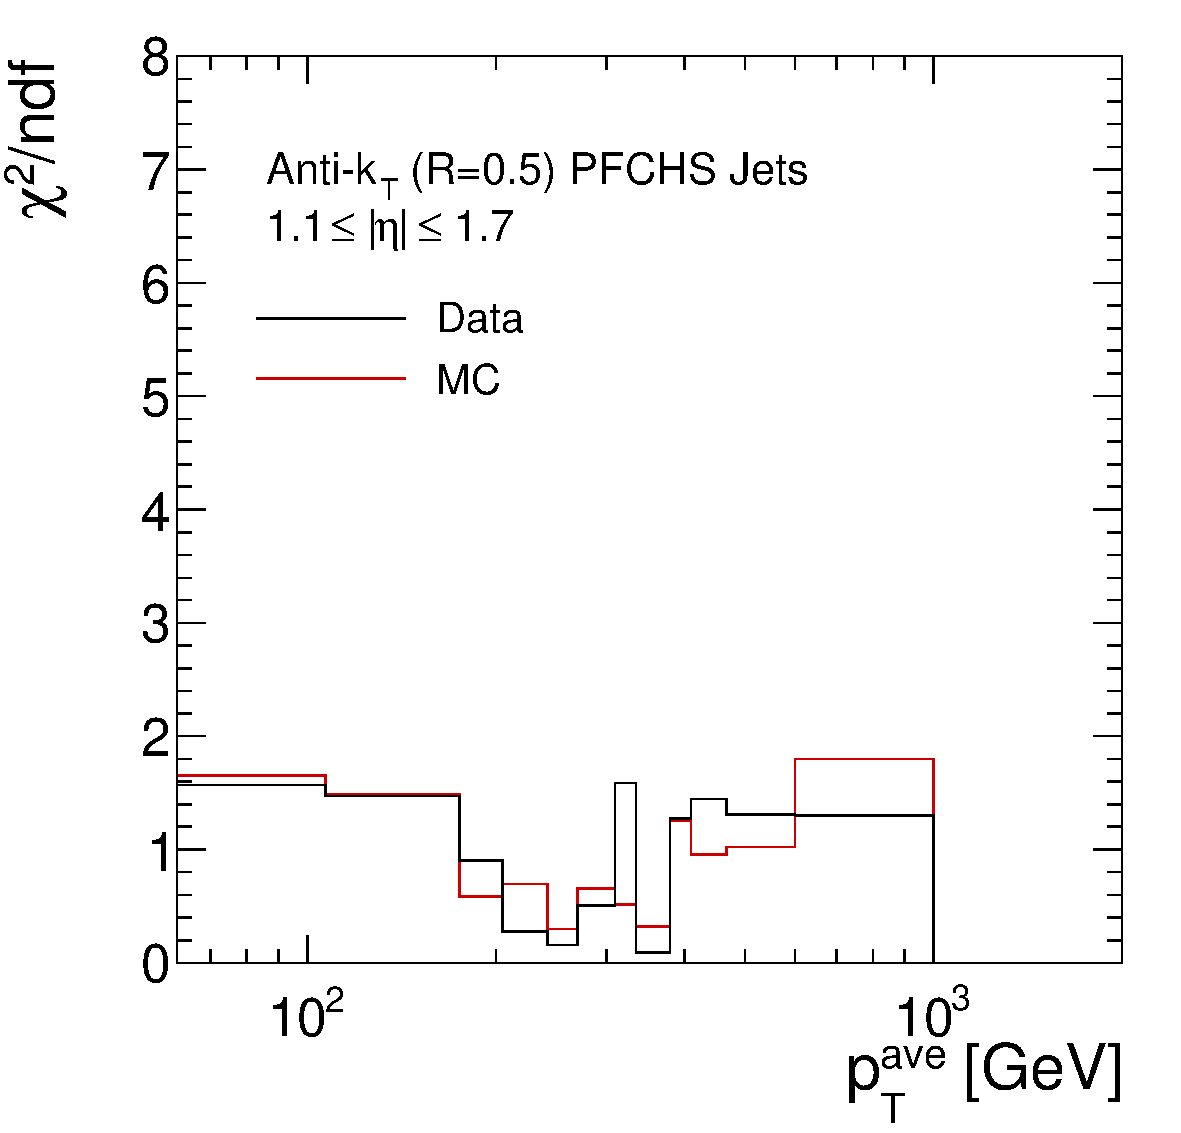
\includegraphics[width=0.49\textwidth]{figures/GoodnessOfFit_Eta2_final_nominal_v4.pdf} &
                \includegraphics[width=0.49\textwidth]{figures/GoodnessOfFit_Eta3_final_nominal_v4.pdf} \\
                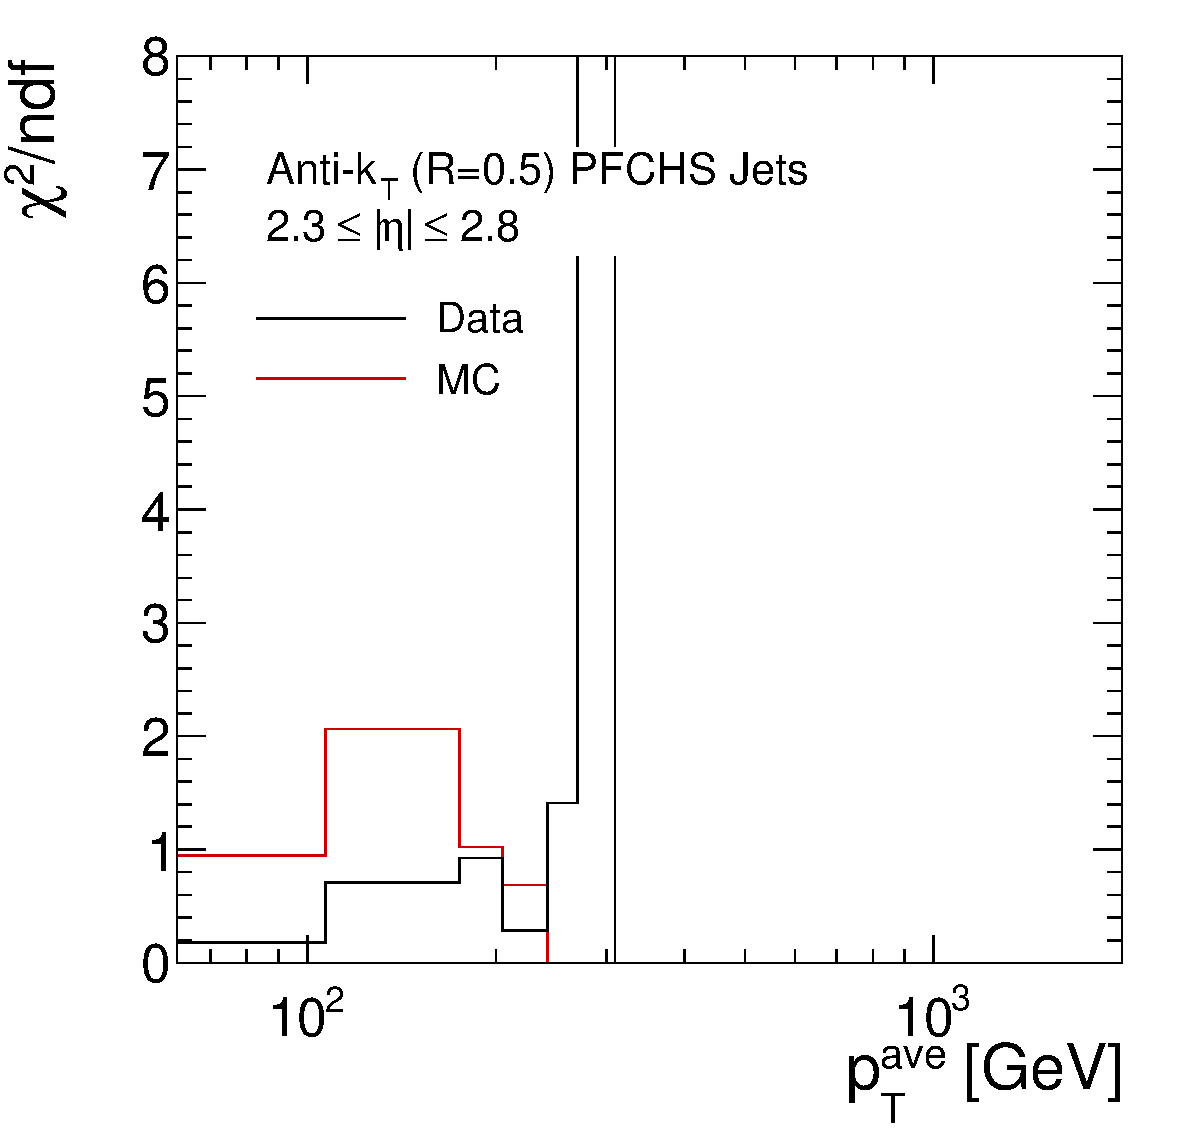
\includegraphics[width=0.49\textwidth]{figures/GoodnessOfFit_Eta4_final_nominal_v4.pdf}
  \end{tabular}
  \caption{Goodness-of-fit test for the extrapolation fits in data and simulation in each $|\eta|$ region as function of $\pt^{ave}$.}
  \label{fig:goodness-of-fit}
\end{figure}

In Fig.~\ref{fig:goodness-of-fit} an overview of a goodness-of-fit test is shown for the extrapolation fits in data and simulation. The resulting $\chi^2$ distribution over the number of degrees of freedom is shown as function of $\pt^{ave}$ for each individual $|\eta|$ interval. In general the fit quality is quite good but worsens for larger $\pt^{ave}$ values. Especially for the higher $\pt^{ave}$ intervals in the central $|\eta|$ regions the statistical uncertainty is rather low and so the fit is very sensitive to even small deviations from a linear behaviour resulting in a minor fit quality. To consider this for the final result a possible non-linearity is covered with a dedicated systematic uncertainty.

\subsection{Correction for Particle-Level Imbalance}
\label{subsec:jer_corrections_pli}
In addition to an imbalance in dijet events caused by the presence of additional jets differences between the momentum of the parton and the corresponding particle-level jet can also arise e.g. from the jet clustering algorithm. This fact is referred to as particle-level imbalance (PLI) and estimated from simulation. \\
\\
The contribution arising from the particle-level imbalance is estimated from the dijet asymmetry at generator level which is defined along with the asymmetry introduced for the resolution measurement itself as
\begin{equation}
  \mathrm{A_{gen}} = \frac{p_{T,1}^{gen} - p_{T,2}^{gen}}{p_{T,1}^{gen} + p_{T,2}^{gen}} 
 \end{equation}
where $p_{T,1}^{gen}$ and $p_{T,2}^{gen}$ refer to the momenta of the two leading generated jets. This distribution is affected the same way as the asymmetry defined in Eq.~\ref{eq:asymmdef} by additional jet activity in the event. Therefore the measured values of $\sigma_{A_{gen}}$ are extrapolated to zero additional jet activity $\alpha_{max} \rightarrow 0$ with the same extrapolation procedure as described in Section~\ref{subsec:jer_corrections_alpha}. Some exemplary extrapolations are shown in Fig.~\ref{fig:extrapol_gen}. \\
\begin{figure}[!tp]
  \centering
  \begin{tabular}{cc}
                \includegraphics[width=0.49\textwidth]{figures/Extrapol_Eta0_pt4_gen_final_nominal_v4.pdf} &
                \includegraphics[width=0.49\textwidth]{figures/Extrapol_Eta0_pt9_gen_final_nominal_v4.pdf}
  \end{tabular}
  \caption{Two examplary extrapolations of measured values for $\sigma_{A,gen}$ in simulation to determine the contribution from PLI.}
  \label{fig:extrapol_gen}
\end{figure}
The contribution due to PLI is then given by
 \begin{equation}
 \label{eq:pli}
 \sigma_\mathrm{PLI} = \sqrt{2} \cdot \sigma_{A_{gen}}(\alpha_{max} \rightarrow 0) \, .
 \end{equation}

\subsection{Results of the Corrections to the Asymmetry}
\label{subsec:jer_corrections_results} 
The results of the various extrapolation fits to determine $ \sigma_{A}(\alpha_{max} \rightarrow 0)$ in data and simulation as well as for the particle-level imbalance are shown together in Fig.~\ref{fig:fit-results} as function of $\pt^{ave}$ for the different $\eta$ regions. 

\begin{figure}[!htp]
  \centering
  \begin{tabular}{cc}
                \includegraphics[width=0.49\textwidth]{figures/Extrapol_Eta0_final_nominal_v4.pdf} &
                \includegraphics[width=0.49\textwidth]{figures/Extrapol_Eta1_final_nominal_v4.pdf} \\
                \includegraphics[width=0.49\textwidth]{figures/Extrapol_Eta2_final_nominal_v4.pdf} &
                \includegraphics[width=0.49\textwidth]{figures/Extrapol_Eta3_final_nominal_v4.pdf} \\
                \includegraphics[width=0.49\textwidth]{figures/Extrapol_Eta4_final_nominal_v4.pdf}
  \end{tabular}
  \caption{Results of extrapolation fits in different $|\eta|$ regions as function of $\pt^{ave}$ for data, simulation and particle-level imbalance.}
  \label{fig:fit-results}
\end{figure}

In order to obtain the jet energy resolution the fit result of the extrapolated $\sigma_\mathrm{PLI}$ is subtracted in quadrature from the measured $\sigma_\mathrm{A}$ after the correction for additional jet activity 
\begin{equation}
\sigma_\mathrm{JER} =  \sqrt{2} \cdot \sigma_{A}(\alpha_{max} \rightarrow 0) \ominus \sigma_\mathrm{PLI} \, .
\end{equation}  
As can be seen in Fig.~\ref{fig:fit-results} the correction due to particle-level imbalance is small compared to the measured asymmetry widths.

\section[Determination of the Data-to-Simulation Ratio]{Determination of the Data-to-Simulation Ratio of the Jet Transverse Momentum Resolution}
\label{sec:jer_ratio_determination}
The measured resolution in data and simulation can be compared after applying all corrections described in Section~\ref{sec:jer_corrections} by calculating the data-to-simulation ratio

\begin{equation}
  c(\mathrm{Data}/\mathrm{MC}) = \frac{ \sigma_\mathrm{JER,\, data}}{ \sigma_\mathrm{JER,\, simulation}} \, .
 \end{equation}

 The resulting distributions as function of $\pt^{ave}$ for various $\eta$ regions are shown in Fig.~\ref{fig:ratio}. As no significant \pt dependence is observed, the ratio is parametrized by a constant fit. The fit result shows in each $|\eta|$ region a value larger than one meaning that the resolution in data is in general worse than in simulation. The constant fit is also visualized in Fig.~\ref{fig:ratio} (red line) together with the statistical uncertainty resulting from the fit (grey shaded area). Due to statistical limitations no data-to-simulation ratio could be determined for the two highest $|\eta|$ intervals. Results are summarized later in Tab~\ref{tab:syst_uncert_summary}. 
 
\begin{figure}[!htp]
  \centering
  \begin{tabular}{cc}
                \includegraphics[width=0.49\textwidth]{figures/ExtrapolRatio_Eta0_with_pli_final_nominal_v4.pdf} &
                \includegraphics[width=0.49\textwidth]{figures/ExtrapolRatio_Eta1_with_pli_final_nominal_v4.pdf} \\
                \includegraphics[width=0.49\textwidth]{figures/ExtrapolRatio_Eta2_with_pli_final_nominal_v4.pdf} &
                \includegraphics[width=0.49\textwidth]{figures/ExtrapolRatio_Eta3_with_pli_final_nominal_v4.pdf} \\
                \includegraphics[width=0.49\textwidth]{figures/ExtrapolRatio_Eta4_with_pli_final_nominal_v4.pdf}
  \end{tabular}
  \caption{Ratio of the resolution in data to the resolution in the QCD sample in different $|\eta|$ regions as function of $\pt^{ave}$ shown together with a constant fit.}
  \label{fig:ratio}
\end{figure}

\section{Validation of the Method}
\label{sec:jer_validation}

\subsection{Validation in Simulated Events}
\label{sec:jer_validation_closure}
In order to test the quality of the method to predict the correct data-to-simulation ratio a so-called closure test on simulated events is performed. \\
Therefore the simulated QCD sample is divided into two sub-samples with equal number of events. In one of the sub-samples the leading corrected jets \footnote{It is necessary to correct all jets which might get relevant for the analysis i.e. become one of the leading three jets. In this analysis the five leading jets in \pt are corrected.} in \pt in each event are smeared with a smearing factor $c$ to increase the \pt resolution, if they have a minimum \pt threshold of $10\,\rm{GeV}$. This means that for each reconstructed jet which has an associated generated jet within a $\Delta R$ cone size of 0.25 the transverse momentum is scaled as follows
\begin{equation}
 p^{'}_{T} = p^{gen}_{T} + c \cdot (p_{T} - p^{gen}_{T}) \, .
\end{equation} 
After the smearing procedure the jets are re-ordered again descendent in \pt.\\
\\
For the closure test the smearing factor has been chosen to be $c = 1.1$ for each $|\eta|$ interval. The ratio of the measured resolution in the smeared QCD sub-sample to the resolution in the unsmeared sub-sample is derived with the asymmetry method including all corrections as described in Section~\ref{sec:jer_corrections}. This should result in a measured ratio of the input value $c\mathrm{(MC_{smeared}/MC)} = 1.1$. The resulting ratios from a constant fit as function of $\pt^{ave}$ in each $|\eta|$ region with statistical uncertainties are summarized in Tab.~\ref{tab:mc_closure}.\\
\\
It can be seen that the input scaling factor of 1.1 is nicely recovered with this procedure within the statistical uncertainties. This allows the conclusion that a potential resolution difference in the ratio when comparing data and simulation can be determined with this approach as well.

\begin{table}[!tp]
\centering
\caption{Ratio $c\mathrm{(MC_{smeared}/MC)}$ of the resolution in the smeared QCD sample to the resolution of the unsmeared QCD sample in various $|\eta|$ regions with statistical uncertainty.}
\label{tab:mc_closure}
% \makebox[\linewidth]{
\begin{tabular}{cccccc}
%\multicolumn{7}{c}{} \\
\hline
 & & & & & \\
 & $|\eta|$ & & $c\mathrm{(MC_{smeared}/MC)}$ & $\rm{stat.}$ & \\
 & & & & & \\
\hline
 & & & & & \\
 & $0.0 - 0.5$ & & 1.11 & $\pm \, 0.01$ & \\
 & & & & & \\
 & $0.5 - 1.1$ & & 1.12 & $\pm \, 0.01$ & \\
 & & & & & \\
 & $1.1 - 1.7$ & & 1.11 & $\pm \, 0.02$ & \\
 & & & & & \\
 & $1.7 - 2.3$ & & 1.06 & $\pm \, 0.04$ & \\
 & & & & & \\
 & $2.3 - 2.8$ & & 1.10 & $\pm \, 0.11$ & \\
 & & & & & \\   
 & $2.8 - 3.2$ & & - & - & \\
 & & & & & \\  
 & $3.2 - 5.0$ & & - & - & \\
 & & & & & \\ 
 \hline 
\end{tabular}%}
\end{table}  

\subsection{Validation of the Measured Data-to-Simulation Ratio}
\label{sec:jer_validation_ratio}
In addition to the closure test on simulated events the measured data-to-simulation ratio can also be directly validated with a similar approach as described in Section~\ref{sec:jer_validation_closure}.\\
For that the individual jet momenta in the simulated QCD sample are scaled with the measured resolution ratio values $c{(\mathrm{Data}/\mathrm{MC})}$ depending on the respective $|\eta|$ region. Applying the measurement procedure of the data-to-simulation ratio again after the smearing procedure one expects to obtain ratios of $c\mathrm{(Data/MC_{smeared})} = 1$ since the resolution differences between data and simulation have been adjusted before. \\
The result of this test is summarized in Tab.~\ref{tab:data_closure} with statistical errors only. A nice agreement with the expected value of 1 is visible even without the consideration of systematic uncertainties in this consistency test. 

\begin{table}[!tp]
\centering
\caption{Ratio $c\mathrm{(Data/MC_{smeared})}$ of the resolution in data to the resolution of the QCD sample smeared with the measured data-to-simulation ratio in various $|\eta|$ regions with statistical uncertainty.}
\label{tab:data_closure}
% \makebox[\linewidth]{
\begin{tabular}{cccccc}
%\multicolumn{7}{c}{} \\
\hline
 & & & & & \\
 & $|\eta|$ & & $c\mathrm{(Data/MC_{smeared})}$ & $\rm{stat.}$ & \\
 & & & & & \\
\hline
 & & & & & \\
 & $0.0 - 0.5$ & & 0.996 & $\pm \, 0.006$ & \\
 & & & & & \\
 & $0.5 - 1.1$ & & 0.997 & $\pm \, 0.006$ & \\
 & & & & & \\
 & $1.1 - 1.7$ & & 0.998 & $\pm \, 0.009$ & \\
 & & & & & \\
 & $1.7 - 2.3$ & & 1.012 & $\pm \, 0.021$ & \\
 & & & & & \\
 & $2.3 - 2.8$ & & 1.001 & $\pm \, 0.064$ & \\
 & & & & & \\   
 & $2.8 - 3.2$ & & - & - & \\
 & & & & & \\  
 & $3.2 - 5.0$ & & - & - & \\
 & & & & & \\ 
 \hline 
\end{tabular}%}
\end{table} 


\section{Systematic Uncertainties}
\label{sec:jer_syst_unc}
In addition to the uncertainty of the resolution measurement due to statictical effects, there are also systematic components which influence the outcome of the data-to-simulation ratio. The different contributions of systematic uncertainties to the measurement are discussed in this section.\\
All systematic uncertainties are determined by evaluating the shift of the data-to-simulation ratio when varying a certain aspect in the measurement procedure. The uncertainty $\delta c$ is calculated by the determination of the ratio for a certain shift $\Delta$ and comparing it to the nominal ratio 
 \begin{equation}
  \delta c{\mathrm{(Data/MC)}} = c{\mathrm{(Data/MC)}_{\Delta}} - c\mathrm{(Data/MC)}
 \end{equation} 
It is symmetrized by taking the average shift, if the variation leads to an upward and a downward shift of the ratio. If the variation results only in an upward or downward shift, the maximum of both is taken and quoted as symmetric uncertainty.  

\begin{description}
 \item[PU reweighting:] The trigger dependent pileup distributions in data which are taken in order to reweight the simulated sample to match the pileup distribution in data are calculated with a nominal minimum bias cross section of $69.4\,\rm{mb}$. In order to evaluate the uncertainty due to this choice the minimum bias cross section is varied to $73.5\,\rm{mb}$ and the pileup scenario of the simulated QCD sample is reweighted to the data distributions obtained with this changed minimum bias cross section. Apart from that the measurement of the data-to-simulation ratio stays the same. \\
 Since the minimum bias cross section is only shifted upwards, the resulting shift in the data-to-simulation ratio is considered as symmetric uncertainty.
 
 \item[Particle-level imbalance:] The measured resolution in data and simulation is corrected for an imbalance at particle level due to out-of-cone showering effects using simulation only. In order to account for the uncertainty on $\sigma_\mathrm{PLI}$ the PLI-correction factor for each measured resolution value is shifted up and down by $25\%$. This means that the changed ratio is calculated as
 \begin{equation}
  c\mathrm{(Data/MC)_{PLI}} = \frac{\sigma_{\mathrm{Data}(\alpha \rightarrow 0)} \ominus (f \cdot \sigma_{\mathrm{PLI}})}{\sigma_{\mathrm{MC}(\alpha \rightarrow 0)} \ominus (f \cdot \sigma_{\mathrm{PLI}})}  
 \end{equation}
with $f=0.75, 1.25$ respectively.
 
 \item[Jet energy scale:] The jet energy scale has been corrected to particle level by the application of certain calibration factors which themselve have an uncertainty assigned. To evaluate the impact of this uncertainty on the data-to-simulation ratio of the resolution all jet momenta in the simulated sample are shifted up and down by the JEC uncertainty. The jet momenta in data stay unchanged.
 
 \item[$\alpha$-spectrum:] To account for additional jet activity in the event the measured width of the asymmetry distributions is extrapolated to zero additional jet activity by a linear function. This linear behaviour is more an empirically found relation than a theoretically fundamental connection. One influencing factor of the linear behaviour is the functional form of the $\alpha$-spectrum. It determines how many events are added to the asymmetry distribution in the next higher $\alpha$ interval and consequently how much the asymmetry distribution is broadened. This can result e.g. in a smaller or bigger slope of the linear function or disturb the linear behaviour.\\
 In order to evaluate the influence of the $\alpha$-spectrum on the data-to-simulation ratio the observed inclusive $\alpha$-spectrum in the simulated sample is reweighted to roughly match that in data. In Fig.~\ref{fig:syst_uncert_alpha_spec} a comparison of the $\alpha$-spectrum in data and simulation is shown. The bottom part displays the ratio $\rm{Data/MC}$. The red curve overlaid in the ratio of the left distribution is used to reweight the events in the simulation. For each event a weight $w(\alpha)$ is calculated according to 
\begin{equation}
w(\alpha) = 0.545 \cdot \mathrm{(erf}(13.5 \cdot \alpha -0.02) +1))
\end{equation}
where erf indicates the error-function~\footnote{ $\mathrm{erf} = \frac{1}{\sqrt{\pi}} \int\limits_{-x}^{x} e^{-t^2} dt$}. This weight is considered as multiplicative factor onto the usual event weight in simulation. 
 \begin{figure}[tp]
  \centering
  \begin{tabular}{cc}
                \includegraphics[width=0.49\textwidth]{figures/Alpha__AfterAsymmHistos.pdf} &
                \includegraphics[width=0.49\textwidth]{figures/AfterReweight_Alpha__AfterAsymmHistos.pdf}
  \end{tabular}
  \caption{Inclusive $\alpha$-spectrum before $(\mathrm{left})$ and after $(\mathrm{right})$ reweighting the $\alpha$-spectrum of the simulated sample. The red curve in the bottom of the left plot illustrates the function used for the $\alpha$-spectrum reweighting.}
  \label{fig:syst_uncert_alpha_spec}
\end{figure}
 
 \item[$\alpha$-range:] The functional form of the $\alpha$-spectrum is only one part of the question concerning the validity of the linear assumption for the extrapolation procedure. There is also the question for which $\alpha$-range this assumption is valid. The choice of the linear function implies that the linear behaviour holds also for small $\alpha$-values where no additional points are measured and up to $\alpha=20$ -- $25\%$. \\
In order to study the linear behaviour of the extrapolation towards smaller $\alpha$-values the minimum \pt cut of 10\gev for the third jet is dropped and an additional $\alpha$-interval 0.0 -- 0.05 is introduced. In Fig.~\ref{fig:syst_uncert_alpha_range} some exemplary extrapolations with the additional $\alpha$-interval are shown. In general the fit quality decreases slightly but is still reasonable (shown in App. \todo{app:fit quality}). The resulting difference in the data-to-simulation ratio is considered as systematic uncertainty.

\begin{figure}[tp]
  \centering
  \begin{tabular}{cc}
                \includegraphics[width=0.49\textwidth]{figures/Extrapol_Eta0_pt4_final_nominal_NoMinPtCutForThirdJet_AddNewAlphaBin_v4.pdf} &
                \includegraphics[width=0.49\textwidth]{figures/Extrapol_Eta0_pt9_final_nominal_NoMinPtCutForThirdJet_AddNewAlphaBin_v4.pdf}
  \end{tabular}
  \caption{Two examplary extrapolations of measured values for $\sigma_\mathrm{A}$ in data and simulation to obtain the result at zero additional jet activity when adding one additional $\alpha$ interval 0.0 --0.05.}
  \label{fig:syst_uncert_alpha_range}
\end{figure}

\item[Non-gaussian tails:] As discussed in Sec.~\ref{sec:jer_application} the width of the asymmetry distribution is calculated as a truncated root-mean-square in order to reject contributions from non-gaussian tails. The truncation was chosen to be 1.5\% for both data and simulation. In general it is possible that the tail contributions in data and simulation differ and consequently do not cancel out in the ratio. In order to evaluate this effect the data-to-simulation ratio is calculated when truncating 5\% of the original distribution instead of 1.5\%.  

\item[Flavour uncertainty:] In general the jet energy resolution for light (u,d,s) and heavy quarks (c,b) can be quite different due to neutrinos occuring in the decay of heavy quarks. This resolution difference related to the quark flavour cancels in principle out in the data-to-simulation ratio, if the flavour composition is the same in data and simulation. Since this is not necessarily the case the impact of heavy quarks produced in gluon splitting processes on the data-to-simulation ratio is evaluated by varying the event weights for events with gluon splitting into heavy quarks.\\
An event is considered as gluon splitting event, if one of the two leading jets has a gluon jet flavour with respect to the physics definition for jet flavour. It is distinguished between gluon splitting into light and heavy jets by identifying if the jet considered as gluon in the physics definition has a b/c-flavour or a light flavour using the algorithmic definition. All events where at least one of the two leading jets is identified as a gluon splitting into heavy quarks get an event weight of 1.5. The data-to-simulation ratio is then derived for the resolution from data to the resolution in the reweighted simulated sample.

\item[Shape of the data-to-simulation ratio:] The data-to-simulation ratio in this measurement is determined by fitting the ratio of $\sigma_\mathrm{JER,\, data}$ to $\sigma_\mathrm{JER,\, simulation}$ with a constant. This assumes that the ratio is flat as function of $\pt^{ave}$. In order to test this assumption one can fit the $\sigma_\mathrm{JER,\, data}$ and $\sigma_\mathrm{JER,\, simulation}$ distributions separately and scale the parameters for data with a certain factor. \\ 
The following function (NSC -- function) is used to fit the resolution in simulation
\begin{equation}
f(\pt) = \sqrt{\frac{N^2}{\pt^{2}} + \frac{S^2}{\pt} + C^2}
\end{equation}
with $\pt=\pt^{ave}$ and parameters N, S and C. If the data-to-simulation ratio is flat as function of $\pt^{ave}$ one expects to find one common scale factor $k_{NSC}$ for the N, S and C parameters to describe the data. A strong influence from e.g. pile-up which might be modelled differently than it actually occurs in data could result in individual scale factors for these parameters. \\
In order to test the assumption of a flat ratio the data points are fitted with the following function 
\begin{equation}
f(\pt) = \sqrt{\frac{(k_{NS} \cdot N)^2}{\pt^{2}} + \frac{(k_{NS} \cdot S)^2}{\pt} + (k_{C} \cdot C)^2} 
\end{equation} 
which uses one scale factor for parameters N and S as well as one scale factor for C while the parameters N, S and C are fixed to the results of the fit to the simulation. The fits are summarized in Fig.~\ref{fig:NSC_Fits_3}.

\begin{figure}[!htp]
  \centering
  \begin{tabular}{cc}
                \includegraphics[width=0.49\textwidth]{figures/Pythia_NSCFit_Eta0_kNS_kC.pdf} &
                \includegraphics[width=0.49\textwidth]{figures/Pythia_NSCFit_Eta1_kNS_kC.pdf}\\
                \includegraphics[width=0.49\textwidth]{figures/Pythia_NSCFit_Eta2_kNS_kC.pdf} &
                \includegraphics[width=0.49\textwidth]{figures/Pythia_NSCFit_Eta3_kNS_kC.pdf} \\
                \includegraphics[width=0.49\textwidth]{figures/Pythia_NSCFit_Eta4_kNS_kC.pdf} 
  \end{tabular}
  \caption{Results of fitting the resolution in data and simulation with the respective NSC-functions in each $|\eta|$ interval.}
  \label{fig:NSC_Fits_3}
\end{figure} 

It turns out that the scale factors $k_{NS}$ and $k_{C}$ are not necessarily equal. In order to see, if such a behaviour is compatible with the measured points for the data-to-simulation ratio, the ratio of the two fitted functions for data and simulation is shown together with the measured values and the constant fit in Fig.~\ref{fig:NSC_Fits_ratio}. 

\begin{figure}[!htp]
  \centering
  \begin{tabular}{cc}
                \includegraphics[width=0.49\textwidth]{figures/Pythia_NSCFit_Eta0_kNS_kC_ratio.pdf} &
                \includegraphics[width=0.49\textwidth]{figures/Pythia_NSCFit_Eta1_kNS_kC_ratio.pdf}\\
                \includegraphics[width=0.49\textwidth]{figures/Pythia_NSCFit_Eta2_kNS_kC_ratio.pdf} &
                \includegraphics[width=0.49\textwidth]{figures/Pythia_NSCFit_Eta3_kNS_kC_ratio.pdf} \\
                \includegraphics[width=0.49\textwidth]{figures/Pythia_NSCFit_Eta4_kNS_kC_ratio.pdf} 
  \end{tabular}
  \caption{Ratio of the results fitting the resolution in data and simulation with the NSC-functions in each $|\eta|$ interval together with the measured ratio and a constant fit.}
  \label{fig:NSC_Fits_ratio}
\end{figure} 

One can see that the ratio derived from the NSC -- fits is also compatible with the measured values for the ratio which means that in principle a trend versus $\pt^{ave}$ could be hidden in the measured points. The difference of the measured scale factors $k_{NS}$ and $k_{C}$ to the central value of the measurement from the constant fit is considered as systematic uncertainty. This also covers possible differences of the scaling factors for jets with very low or very high transverse momenta which can not be directly measured in this analysis. As the NSC-Fits in the higher $|\eta|$ intervals suffer from the low number of events there, a 2\% uncertainty on the shape of the data-to-simulation ratio is considered for all $|\eta|$ intervals.

\end{description}

A summary of the data-to-simulation ratios measured with this method together with all systematic uncertainties considered for the ratio is given in Tab~\ref{tab:syst_uncert_summary}. 

\begin{table}[!htp]
\centering
\caption{Summary of the measured data-to-simulation ratios $c\mathrm{(Data/MC)}$ with statistical uncertainty and systematic uncertainty for each uncertainty source in different $|\eta|$ regions.}
\label{tab:syst_uncert_summary}
% \makebox[\linewidth]{
\begin{tabular}{lcccccccc}
%\multicolumn{10}{c}{} \\
\hline
 %& & \multicolumn{7}{c}{} \\
 %& & \multicolumn{7}{c}{$|\eta|$} \\
 %& & \multicolumn{7}{c}{} \\
\hline
 & & & & & & & & \\
 & & $0.0 - 0.5$ & $0.5 - 1.1$ & $1.1 - 1.7$ & $1.7 - 2.3$ & $2.3 - 2.8$ & $2.8 - 3.2$ & $3.2 - 5.0$ \\
 & & & & & & & & \\
 \hline
 & & & & & & & & \\
 $c\mathrm{(Data/MC)}$ & & 1.077 & 1.100 & 1.119 & 1.205 & 1.145 & - & - \\
 & & & & & & & & \\
 Stat. uncertainty & & $\pm$ 0.007 & $\pm$ 0.006 & $\pm$ 0.010 & $\pm$ 0.027 & $\pm$ 0.078 & - & - \\
 & & & & & & & & \\
\hline
 & & & & & & & & \\
 PU reweighting & & $\pm$ 0.004 & $\pm$ 0.003 & $\pm$ 0.004 & $\pm$ 0.004 & $\pm$ 0.013 & - & -  \\
 & & & & & & & & \\
 Particle-level imbalance & & $\pm$ 0.004 & $\pm$ 0.005 &$\pm$  0.005 & $\pm$ 0.015 & $\pm$ 0.010 & - & - \\
 & & & & & & & & \\
 Jet energy scale & & $\pm$ 0.005 & $\pm$ 0.007 & $\pm$ 0.008 & $\pm$ 0.015 & $\pm$ 0.020 & - & - \\
 & & & & & & & & \\
 $\alpha$-spectrum & & $\pm$ 0.004 & $\pm$ 0.007 & $\pm$ 0.004 & $\pm$ 0.006 & $\pm$ 0.003 & - & - \\
 & & & & & & & & \\
 $\alpha$-range & & $\pm$ 0.005 & $\pm$ 0.009 & $\pm$ 0.004 & $\pm$ 0.011 & $\pm$ 0.012 & - & - \\
 & & & & & && &  \\
 Non-gaussian tails & & $\pm$ 0.004 & $\pm$ 0.003 & $\pm$ 0.003 & $\pm$ 0.013 &$\pm$ 0.007 & - & - \\
 & & & & & & & & \\ 
 Jet Flavour & & $\pm$ 0.007 & $\pm$ 0.004 & $\pm$ 0.005 & $\pm$ 0.006 & $\pm$ 0.003 & - & - \\
 & & & & & & & & \\ 
 Ratio shape & & $\pm$ 0.022 & $\pm$ 0.022 & $\pm$ 0.022 & $\pm$ 0.024 & $\pm$ 0.023 & - & - \\
 & & & & & & & & \\ 
\hline
 & & & & & & & & \\
 Total syst. uncertainty & & $\pm$ 0.025 & $\pm$ 0.027 & $\pm$ 0.026 & $\pm$ 0.038 & $\pm$ 0.038 & - & - \\
 & & & & & & & & \\ 
\hline
\end{tabular}%}
\end{table} 

\section{Extension of the Method to the Forward Detector Region}
\label{sec:jer_forward_extension}
The measurement presented until here is based on the requirement that the two leading jets in an event belong both to the same $|\eta|$ region. This means that the resolution of these two jets is the same and results in the relation that $\frac{\sigma (p_{T})}{\langle p_{T} \rangle} = \sqrt{2} \cdot \sigma_{A}$. This requirement of $|\eta_{\mathrm{jet},1}|$ = $|\eta_{\mathrm{jet},2}|$ reduces significantly the available number of events especially in the forward region of the detector as the jets in these events have low transverse momenta and consequently have to be triggered by the lowest $\pt^{ave}$ triggers which are highly prescaled. Thus for the intervals $|\eta| > 2.8$ no data-to-simulation ratio could be determined. \\
\\
In order to extend the analysis such that a measurement in the forward region of the detector is also possible one can drop the requirement that $|\eta_{\mathrm{jet},1}|$ = $|\eta_{\mathrm{jet},2}|$ and select events where the two leading jets belong to different pseudorapidity regions. The resolution $\sigma (p_{T}^{\mathrm{jet, probe}})$ in a probe interval $|\eta_\mathrm{probe}|$ can then be measured, if the resolution $\sigma (p_{T}^{\mathrm{jet, ref}})$ in a reference interval $|\eta_\mathrm{ref}|$ is already known. \\
\\
Starting again with the relation in Eq.~\ref{eq:asymm_first}, it can be shown that for $\langle p_{T,\mathrm{probe}} \rangle = \langle p_{T,\mathrm{ref}} \rangle = \langle \pt \rangle$ and $\sigma (p_{T,\mathrm{probe}}) \neq \sigma (p_{T,\mathrm{ref}})$ one obtains the relation
\begin{equation}
 \label{eq:asymm_forward}
  \frac{\sigma (p_{T, \mathrm{probe}})}{\langle p_{T} \rangle} = \sqrt{4 \cdot \sigma_{A({|\eta_{\mathrm{probe}|} \neq |\eta_{\mathrm{ref}}|)}} - \left(\frac{\sigma (p_{T, \mathrm{ref}})}{\langle p_{T} \rangle} \right)^2} 
 \end{equation}
where $\sigma_{A({|\eta_{\mathrm{probe}|} \neq |\eta_{\mathrm{ref}}|)}}$ is the width of the asymmetry calculated from the two leading jets in an event of which one jet is in a reference $|\eta|$ interval for which the resolution has been already measured with the same-$|\eta|$ requirement and the probe jet belonging to another $|\eta|$ region. The asymmetry width is taken after the correction for additional jet activity and the particle-level imbalance determined from $\sigma_{A, \mathrm{gen} ({|\eta_{\mathrm{probe}|} \neq |\eta_{\mathrm{ref}}|)}}$. The reference interval is preferred to be in the central detector region where the statistical precision from the same-$|\eta|$ measurement has already been sufficient. The statistical uncertainty of $\frac{\sigma (p_{T, \mathrm{ref}})}{{\langle p_{T} \rangle}}$ is propagated to the statistical uncertainty of $\frac{\sigma (p_{T, \mathrm{probe}})}{\langle p_{T} \rangle}$. \\
\\
As long as both jets belong to the same $|\eta|$ region residual effects from jet energy scale differences in data and simulation affect both jets the same way and should not have an impact on the resolution measurement. Since residual effects from the jet energy scale where the mean of the asymmetry is shifted and not exactly zero become more important, if both jets belong to different probe and reference intervals, the asymmetry is defined as
\begin{equation}
\label{eq:forwardasymmdef}
  \mathrm{A} = \frac{p_{\mathrm{T,probe}} - p_{\mathrm{T,ref}}}{p_{\mathrm{T,probe}} + p_{\mathrm{T,ref}}} 
 \end{equation}
for the reference-and-probe interval measurement for the transverse momenta $p_{\mathrm{T,ref}}$ and $p_{\mathrm{T,probe}}$ of the reference and probe jet, respectively. Accordingly, in the determination of the asymmetry width $\sigma_{A}$ the mean of the distribution $A_\mathrm{mean}$ is also estimated and the width calculated as
\begin{equation}
\label{eq:forwardasymmwidthdef}
  \sigma_{A} = \mathrm{RMS}_{98.5\%} = \sqrt{\frac{1}{n} \cdot \sum_{i}(A_i-A_\mathrm{mean})^2} 
 \end{equation}
with the number of possible values $n$ for the individual asymmetry values $A_i$ where the sum over $i$ includes all values such that $98.5\%$ of the total asymmetry distribution are covered symmetric around the mean.\\
\\
The measurement with the reference-and-probe interval selection is performed taking the three innermost $|\eta|$ regions 0.0 -- 0.5, 0.5 -- 1.1 and 1.1 -- 1.7 as reference intervals each. This allows a measurement of the data-to-simulation ratio also in the intervals 2.8 -- 3.2 and 3.2 -- 5.0. In addition, it provides for the innermost $|\eta|$ intervals an enhancement of the available number of events and thus a further reduction of the statistical uncertainties.\\
\\
The systematic uncertainties of the two new measurements are evaluated the same way as for the same-$|\eta|$ measurement by varying a certain aspect in the determination of the data-to-simulation ratio and taking the deviation from the nominal ratio as uncertainty. The variation is done for the $\sigma_{A({|\eta_{\mathrm{probe}|} \neq |\eta_{\mathrm{ref}}|)}}$ value as well as for $\frac{\sigma (p_{T, \mathrm{ref}})}{{\langle p_{T} \rangle}}$ for each uncertainty source.\\
\\
A summary of the resulting data-to-simulation ratios determined in the measurements with the two different reference intervals and the corresponding uncertainties is shown in Table~\ref{tab:syst_uncert_summary_forward_central} for $|\eta_\mathrm{ref}|$ = 0.0 -- 0.5, Table~\ref{tab:syst_uncert_summary_forward_nexttocentral} for $|\eta_\mathrm{ref}|$ = 0.5 -- 1.1 and Table~\ref{tab:syst_uncert_summary_forward_secondnexttocentral} for $|\eta_\mathrm{ref}|$ = 1.1 -- 1.7, respectively.

\begin{table}[!hp]
\centering
\caption{Summary of the measurement with reference bin $|\eta| = 0.0 - 0.5$ showing the nominal data-to-simulation ratio $c\mathrm{(Data/MC)}$ with statistical uncertainty and systematic uncertainty for each uncertainty source in different $|\eta|$ regions.}
\label{tab:syst_uncert_summary_forward_central}
% \makebox[\linewidth]{
\begin{tabular}{lcccccccc}
%\multicolumn{9}{c}{} \\
\hline
% & & \multicolumn{7}{c}{} \\
% & & \multicolumn{7}{c}{$|\eta_\mathrm{ref}| = 0.0 - 0.5$} \\
% & & \multicolumn{7}{c}{} \\
% & & \multicolumn{7}{c}{$|\eta_\mathrm{probe}|$} \\
% & & \multicolumn{7}{c}{} \\
\hline
 & & & & & & & & \\
 & & $0.0 - 0.5$ & $0.5 - 1.1$ & $1.1 - 1.7$ & $1.7 - 2.3$ & $2.3 - 2.8$ & $2.8 - 3.2$ & $3.2-5.0$ \\
 & & & & & & & & \\
\hline
 & & & & & & & & \\
 $c\mathrm{(Data/MC)}$ & & - & 1.106 & 1.133 & 1.227 & 1.253 & 1.410 & 1.171 \\
 & & & & & & & & \\
 Stat. uncertainty & & - & $\pm$ 0.008 & $\pm$ 0.009 & $\pm$ 0.025 & $\pm$ 0.047 & $\pm$ 0.068 & $\pm$ 0.116 \\
 & & & & & & & & \\
\hline
 & & & & & & & & \\
 PU reweighting & & - & $\pm$ 0.002 & $\pm$ 0.001 & $\pm$ 0.001 & $\pm$ 0.021 & $\pm$ 0.025 & $\pm$ 0.007 \\
 & & & & & & & & \\
 Particle-level imbalance & & - & $\pm$ 0.005 & $\pm$ 0.005 & $\pm$ 0.008 & $\pm$ 0.009 & $\pm$ 0.006 & $\pm$ 0.004 \\
 & & & & & & & & \\
 Jet energy scale & & - & $\pm$ 0.006 & $\pm$ 0.010 & $\pm$ 0.021 & $\pm$ 0.034 & $\pm$ 0.022 & $\pm$ 0.066 \\
 & & & & & & & & \\
 $\alpha$-spectrum & & - & $\pm$ 0.010 & $\pm$ 0.006 & $\pm$ 0.011 & $\pm$ 0.006 & $\pm$ 0.009 & $\pm$ 0.012 \\
 & & & & & & & & \\
 $\alpha$-range & & - & $\pm$ 0.010 & $\pm$ 0.014 & $\pm$ 0.046 & $\pm$ 0.089 & $\pm$ 0.015 & $\pm$ 0.018  \\
 & & & & & & & & \\
 Non-gaussian tails & & - & $\pm$ 0.001 & $\pm$ 0.007 & $\pm$ 0.005  & $\pm$ 0.044  & $\pm$ 0.046 & $\pm$ 0.029 \\
 & & & & & & & & \\ 
 Jet Flavour & & - & $\pm$ 0.004 & $\pm$ 0.004 & $\pm$ 0.001 & $\pm$ 0.021 & $\pm$ 0.013 & $\pm$ 0.008 \\
 & & & & & & & & \\ 
 Ratio shape & & - & $\pm$ 0.022 & $\pm$ 0.023 & $\pm$ 0.025 & $\pm$ 0.025 & $\pm$ 0.028 & $\pm$ 0.023 \\
 & & & & & & & & \\ 
\hline
 & & & & & & & & \\
 Total syst. uncertainty & & - & $\pm$ 0.028 & $\pm$ 0.030 & $\pm$ 0.058 & $\pm$ 0.112 & $\pm$ 0.067 & $\pm$ 0.079 \\
 & & & & & & & & \\ 
\hline
\end{tabular}%}
\end{table} 

\begin{table}[!hp]
\centering
\caption{Summary of the measurement with reference bin $|\eta| = 0.5 - 1.1$ showing the nominal data-to-simulation ratio $c\mathrm{(Data/MC)}$ with statistical uncertainty and systematic uncertainty for each uncertainty source in different $|\eta|$ regions.}
\label{tab:syst_uncert_summary_forward_nexttocentral}
% \makebox[\linewidth]{
\begin{tabular}{lcccccccc}
%\multicolumn{9}{c}{} \\
\hline
% & & \multicolumn{7}{c}{} \\
% & & \multicolumn{7}{c}{$|\eta_\mathrm{ref}| = 0.5 - 1.1$} \\
% & & \multicolumn{7}{c}{} \\
% & & \multicolumn{7}{c}{$|\eta_\mathrm{probe}|$} \\
% & & \multicolumn{7}{c}{} \\
\hline
 & & & & & & & & \\
 & & $0.0 - 0.5$ & $0.5 - 1.1$ & $1.1 - 1.7$ & $1.7 - 2.3$ & $2.3 - 2.8$ & $2.8 - 3.2$ & $3.2-5.0$ \\
 & & & & & & & & \\
\hline
 & & & & & & & & \\
 $c\mathrm{(Data/MC)}$ & & 1.081 & - & 1.111 & 1.206 & 1.300 & 1.356 & 0.829 \\
 & & & & & & & & \\
 Stat. uncertainty & & $\pm$ 0.008 & - & $\pm$ 0.009 & $\pm$ 0.023 & $\pm$ 0.047 & $\pm$ 0.058 & $\pm$ 0.082 \\
 & & & & & & & & \\
\hline
 & & & & & & & & \\
 PU reweighting & & $\pm$ 0.001 & - & $\pm$ 0.003 & $\pm$ 0.005 & $\pm$ 0.002 & $\pm$ 0.024 & $\pm$ 0.039 \\
 & & & & & & & & \\
 Particle-level imbalance & & $\pm$ 0.005 & - & $\pm$ 0.005 & $\pm$ 0.010 & $\pm$ 0.017 & $\pm$ 0.009 & $\pm$ 0.021 \\
 & & & & & & & & \\
 Jet energy scale & & $\pm$ 0.008 & - & $\pm$ 0.009 & $\pm$ 0.021 & $\pm$ 0.009 & $\pm$ 0.061 & $\pm$ 0.134 \\
 & & & & & & & & \\
 $\alpha$-spectrum & & $\pm$ 0.007 & - & $\pm$ 0.004 & $\pm$ 0.003 & $\pm$ 0.008 & $\pm$ 0.036 & $\pm$ 0.002 \\
 & & & & & & & & \\
 $\alpha$-range & & $\pm$ 0.004 & - & $\pm$ 0.012 & $\pm$ 0.016 & $\pm$ 0.043 & $\pm$ 0.048 & $\pm$ 0.041 \\
 & & & & & & & & \\
 Non-gaussian tails & & $\pm$ 0.004 & - & $\pm$ 0.008 & $\pm$ 0.010 & $\pm$ 0.061 & $\pm$ 0.023 & $\pm$ 0.012 \\
 & & & & & & & & \\ 
 Jet Flavour & & $\pm$ 0.005 & - & $\pm$ 0.007 & $\pm$ 0.009 & $\pm$ 0.013 & $\pm$ 0.042 & $\pm$ 0.007 \\
 & & & & & & & & \\ 
 Ratio shape & & $\pm$ 0.022 & - & $\pm$ 0.022 & $\pm$ 0.024 & $\pm$ 0.026 & $\pm$ 0.027 & $\pm$ 0.017 \\
 & & & & & & & & \\ 
\hline
 & & & & & & & & \\
 Total syst. uncertainty & & $\pm$ 0.026 & - & $\pm$ 0.030 & $\pm$ 0.039 & $\pm$ 0.082 & $\pm$ 0.105 & $\pm$ 0.149 \\
 & & & & & & & & \\ 
\hline
\end{tabular}%}
\end{table} 

\begin{table}[!hp]
\centering
\caption{Summary of the measurement with reference bin $|\eta| = 1.1 - 1.7$ showing the nominal data-to-simulation ratio $c\mathrm{(Data/MC)}$ with statistical uncertainty and systematic uncertainty for each uncertainty source in different $|\eta|$ regions.}
\label{tab:syst_uncert_summary_forward_secondnexttocentral}
% \makebox[\linewidth]{
\begin{tabular}{lcccccccc}
%\multicolumn{9}{c}{} \\
\hline
% & & \multicolumn{7}{c}{} \\
% & & \multicolumn{7}{c}{$|\eta_\mathrm{ref}| = 1.1 - 1.7$} \\
% & & \multicolumn{7}{c}{} \\
% & & \multicolumn{7}{c}{$|\eta_\mathrm{probe}|$} \\
% & & \multicolumn{7}{c}{} \\
\hline
 & & & & & & & & \\
 & & $0.0 - 0.5$ & $0.5 - 1.1$ & $1.1 - 1.7$ & $1.7 - 2.3$ & $2.3 - 2.8$ & $2.8 - 3.2$ & $3.2-5.0$ \\
 & & & & & & & & \\
\hline
 & & & & & & & & \\
 $c\mathrm{(Data/MC)}$ & & 1.084 & 1.082 & - & 1.189 & 1.250 & 1.432 & 1.137 \\
 & & & & & & & & \\
 Stat. uncertainty & & $\pm$ 0.012 & $\pm$ 0.012 & - & $\pm$ 0.031 & $\pm$ 0.051 & $\pm$ 0.066 & $\pm$ 0.105 \\
 & & & & & & & & \\
\hline
 & & & & & & & & \\
 PU reweighting & & $\pm$ 0.005 & $\pm$ 0.004 & - & $\pm$ 0.024 & $\pm$ 0.001 & $\pm$ 0.002 & $\pm$ 0.029 \\
 & & & & & & & & \\
 Particle-level imbalance & & $\pm$ 0.004 & $\pm$ 0.004 & - & $\pm$ 0.016 & $\pm$ 0.017 & $\pm$ 0.019 & $\pm$ 0.006 \\
 & & & & & & & & \\
 Jet energy scale & & $\pm$ 0.012 & $\pm$ 0.010 & - & $\pm$ 0.029 & $\pm$ 0.041 & $\pm$ 0.055 & $\pm$ 0.018 \\
 & & & & & & & & \\
 $\alpha$-spectrum & & $\pm$ 0.006 & $\pm$ 0.008 & - & $\pm$ 0.019 & $\pm$ 0.006 & $\pm$ 0.019 & $\pm$ 0.009 \\
 & & & & & & & & \\
 $\alpha$-range & & $\pm$ 0.016 & $\pm$ 0.022 & - & $\pm$ 0.036 & $\pm$ 0.032 & $\pm$ 0.016 & $\pm$ 0.048 \\
 & & & & & & & & \\
 Non-gaussian tails & & $\pm$ 0.010 & $\pm$ 0.010 & - & $\pm$ 0.005 & $\pm$ 0.018 & $\pm$ 0.012 & $\pm$ 0.047 \\
 & & & & & & & & \\ 
 Jet Flavour & & $\pm$ 0.005 & $\pm$ 0.007 & - & $\pm$ 0.012 & $\pm$ 0.015 & $\pm$ 0.031 & $\pm$ 0.054 \\
 & & & & & & & & \\ 
 Ratio shape & & $\pm$ 0.022 & $\pm$ 0.022 & - & $\pm$ 0.024 & $\pm$ 0.025 & $\pm$ 0.029 & $\pm$ 0.023 \\
 & & & & & & & & \\ 
\hline
 & & & & & & & & \\
 Total syst. uncertainty & & $\pm$ 0.033 & $\pm$ 0.036 & - & $\pm$ 0.063 & $\pm$ 0.065 & $\pm$ 0.077 & $\pm$ 0.096 \\
 & & & & & & & & \\ 
\hline
\end{tabular}%}
\end{table}  

\section{Measurement for simulated events obtained with the \herwig generator} 
\label{sec:jer_result_herwig}
In order to test if the data-to-simulation ratio is generator independent the ratio is also derived for simulated events generated with \herwig \footnote{The \herwig sample is $\mathrm{/QCD\_Pt-15to3000\_TuneEE3C\_Flat\_8TeV\_herwigpp}$ created in the series $\mathrm{/Summer12\_DR53X-PU\_S10\_START53\_V7A-v1/AODSIM}$}.\\
Fig.~\ref{fig:control_plots_herwig} shows the inclusive $\pt^{ave}$ spectrum compared in data and simulation for simulated events taken from \herwig. \\

\begin{figure}[!hp]
  \centering
  \begin{tabular}{c}
                \includegraphics[width=0.49\textwidth]{figures/HerwigPtAve__AfterAsymmHistos.pdf}
  \end{tabular}
  \caption{Inclusive $\pt^{ave}$ spectrum of events after the event selection in data and in simulated events generated with \herwig.}
  \label{fig:control_plots_herwig}
\end{figure}
The agreement of the $\pt^{ave}$ spectrum between data and simulation looks reasonable and is similar to the spectrum in simulated events from \pythia.\\
\\ 
The resulting data-to-simulation ratios for \herwig from the different measurements together with statistical uncertainties are summarized in Tab.~\ref{tab:result_herwig} 
\begin{table}[!htp]
\centering
\caption{Measured data-to-simulation ratio in various $|\eta|$ regions with statistical uncertainty for simulated events obtained with the \herwig generator.}
\label{tab:result_herwig}
% \makebox[\linewidth]{
\begin{tabular}{ccccccccc}
%\multicolumn{10}{c}{} \\
\hline
  & & & & & & & &\\
 & & & $|\eta_{1}|$ = $|\eta_{2}|$ & $|\eta_\mathrm{ref}|$ = 0.0 - 0.5 & $|\eta_\mathrm{ref}|$ = 0.5 - 1.1 & $|\eta_\mathrm{ref}|$ = 1.1 - 1.7 & &\\
 & & & & & & & &\\	
 & $|\eta|$ & & $c\mathrm{(Data/MC)}$ & $c\mathrm{(Data/MC)}$ & $c\mathrm{(Data/MC)}$ & $c\mathrm{(Data/MC)}$ & \\
& & & & & & & &\\
\hline
 & & & & & & & &\\
 & $0.0 - 0.5$ & & 1.090 $\pm \, 0.008$ & -                    &  1.091 $\pm \, 0.011$ & 1.129 $\pm \, 0.017$ & \\
 & & & & & & & &\\
 & $0.5 - 1.1$ & & 1.107 $\pm \, 0.008$ & 1.111 $\pm \, 0.010$ & -                     & 1.121 $\pm \, 0.016$ & \\
 & & & & & & & &\\
 & $1.1 - 1.7$ & & 1.117 $\pm \, 0.013$ & 1.177 $\pm \, 0.013$ & 1.149 $\pm \, 0.012$  & -                    & \\
 & & & & & & & &\\
 & $1.7 - 2.3$ & & 1.297 $\pm \, 0.038$ & 1.212 $\pm \, 0.035$ & 1.229 $\pm \, 0.033$  & 1.187 $\pm \, 0.041$ & \\
 & & & & & & & &\\
 & $2.3 - 2.8$ & & 1.085 $\pm \, 0.080$ & 1.231 $\pm \, 0.072$ & 1.178 $\pm \, 0.061$  & 1.363 $\pm \, 0.087$ & \\
 & & & & & & & &\\
 & $2.8 - 3.2$ & & -                    & 1.368 $\pm \, 0.094$ & 1.259 $\pm \, 0.061$  & 1.488 $\pm \, 0.112$ & \\
 & & & & & & & &\\
 & $3.2 - 5.0$ & & -                    & 1.245 $\pm \, 0.158$ & 1.124 $\pm \, 0.128$  & 1.324 $\pm \, 0.215$ & \\
 & & & & & & & &\\
\hline
\end{tabular}%}
\end{table} 
In general, the obtained data-to-simulation ratios for \herwig are quite similar to that obtained from \pythia while some further discussion can be found in Sec.~\ref{subsec:jer_combination}.

\section{Results}
\label{sec:jer_results}

\subsection{Determination of a combined result}
\label{subsec:jer_combination}
In order to determine one data-to-simulation ratio for each $|\eta|$ region the results obtained from the individual measurements are combined into one result. This combination is for all $|\eta|$ regions -- except for the very last $|\eta|$ region ranging from 3.2 -- 5.0 which is discussed separately -- derived from the measurements done with simulated events from \pythia while the \herwig results are only used as cross check. The combined result for all $|\eta|$ regions up to 3.2 using events from \herwig are shown in Appendix \todo{app:combination herwig}.\\
The combined data-to-simulation ratios are calculated as weighted mean from the individual measurements with the same-$|\eta|$ requirement and the three central-forward combinations. Each measurement is weighted by its' statistical uncertainty. For the evaluation of the systematic uncertainties considered for the combined result the systematic shift of the weighted mean caused by the systematic shifts of the single measurements is determined. This means that for each uncertainty source the individual up and down shifts to the nominal ratio of each measurement are taken and combined as the weighted mean using the statistical uncertainty just as for the nominal mean. Consequentially, the difference of each systematically shifted weighted mean to the nominal weighted mean is the respective systematic uncertainty for the combination. The total systematic uncertainty quoted for the weighted mean of the data-to-simulation ratio is the average of the individual systematic uncertainties in each $|\eta|$ interval.\\
The $|\eta|$ region from 3.2 -- 5.0 covering the most forward region of the detector -- namely the hadronic forward -- behaves a bit special compared to the others. In contrast to the other $|\eta|$ regions, the individual measurements from \pythia and \herwig have a very large spread of 0.83 up to 1.32 in this particular interval. If one wants to have one combined ratio factor for this interval, it is in this case reasonable to use all six individual measurements from \pythia as well as from \herwig to find a result which covers all of these partly very different ratios. If one combines the measurements following the same procedure as described for the other intervals and taking the systematic uncertainty from the combined \pythia results the combined total result would be 1.056 $\pm$ 0.048 (stat. unc.) $\pm$ 0.079 (syst. unc.) (= 0.092 total unc.). In order to test the consistency of this combined value with the single measurements the $\chi^2/ndf$ is calculated which results in  $\chi^2/\mathrm{ndf} = 4.3$. This shows that the obtained total uncertainty is too small to reasonably cover all individual results. Hence the systematic uncertainty is increased to a value of $\pm$ 0.185 which gives a total uncertainty of $\pm$ 0.191 and results in a $\chi^2/\mathrm{ndf} = 1.0$ such that the single measurements are well represented by this combined result.\\
The obtained data-to-simulation ratios for different $|\eta|$ regions are summarized in Tab.~\ref{tab:result} together with the statistical and systematic uncertainties. In addition, Fig.~\ref{fig:result_2012} shows the measured ratios with the total uncertainty which is the quadratic sum of the statistical and systematic uncertainties. \\
The determined ratios vary from 1.06 to 1.40 and are larger than one in all detector parts. Possible sources of this difference can be e.g. mismodelled noise effects or inhomogenities of the detector.

\begin{table}[!hp]
\centering
\caption{Measured data-to-simulation ratio in various $|\eta|$ regions with statistical and systematic uncertainty as well as the total uncertainty.}
\label{tab:result}
% \makebox[\linewidth]{
\begin{tabular}{cccc|cc|cc}
%\multicolumn{9}{c}{} \\
\hline
 & & & & & & &\\
 & $|\eta|$ & & $c\mathrm{(Data/MC)}$ & $\rm{stat.}$ & $\rm{syst.}$ & $\rm{tot.}$\\
 & & & & & & &\\
\hline
 & & & & & & &\\
 & $0.0 - 0.5$ & & 1.079 & $\pm \, 0.005$ & $\pm \, 0.026$ & $\pm \, 0.026$ \\
 & & & & & & &\\
 & $0.5 - 1.1$ & & 1.099 & $\pm \, 0.005$ & $\pm \, 0.028$ & $\pm \, 0.028$ \\
 & & & & & & &\\
 & $1.1 - 1.7$ & & 1.121 & $\pm \, 0.005$ & $\pm \, 0.029$ & $\pm \, 0.029$ \\
 & & & & & & &\\
 & $1.7 - 2.3$ & & 1.208 & $\pm \, 0.013$ & $\pm \, 0.045$ & $\pm \, 0.046$ \\
 & & & & & & &\\
 & $2.3 - 2.8$ & & 1.254 & $\pm \, 0.026$ & $\pm \, 0.056$ & $\pm \, 0.062$ \\
 & & & & & & &\\
 & $2.8 - 3.2$ & & 1.395 & $\pm \, 0.036$ & $\pm \, 0.051$ & $\pm \, 0.063$ \\
 & & & & & & &\\
 & $3.2 - 5.0$ & & 1.056 & $\pm \, 0.048$ & $\pm \, 0.185$ & $\pm \, 0.191$ \\
 & & & & & & &\\
\hline
\end{tabular}%}
\end{table} 

\begin{figure}[!hp]
  \centering
  \begin{tabular}{c}
                \includegraphics[width=0.6\textwidth]{figures/JER_2012_final_combination_v1.pdf}
  \end{tabular}
  \caption{Measured data-to-simulation ratio in various $|\eta|$ regions displayed with total uncertainty.}
  \label{fig:result_2012}
\end{figure}
 
\subsection{Comparison to Other Measurements}
\label{subsec:jer_results_comparison}
Earlier analyses using dijet events for data collected at $\sqrt{s}=7$\tev have obtained similar results showing data-to-simulation ratios greater than one. A complementary approach is followed using $\gamma +\rm{jet}$ events which offer a very precise opportunity to measure the jet resolution due to the excellent resolution of the photon energy. A comparison of the numbers presented here to the latest $\sqrt{s}=7$\tev results from dijet events~\cite{thesis:Schroeder} and $\sqrt{s}=8$\tev results for $\gamma +\rm{jet}$ measurements~\cite{CMS-AN-2013-179} are shown together in Fig.~\ref{fig:result_comparison}.

\begin{figure}[!hp]
  \centering
  \begin{tabular}{cc}
                \includegraphics[width=0.49\textwidth]{figures/JER_2012_compPhoton_final_combination_v1.pdf} &
                \includegraphics[width=0.49\textwidth]{figures/JER_2012_comp2011_final_combination_v1.pdf}
  \end{tabular}
  \caption{Measured data-to-simulation ratio in various $|\eta|$ regions displayed with total uncertainty. Comparison to results obtained for $\sqrt{s}=8$\tev data from $\gamma +\rm{jet}$ events $(\mathrm{left})$ and to $\sqrt{s}=7$\tev data from dijet events $(\mathrm{right})$.}
  \label{fig:result_comparison}
\end{figure}

The results obtained from different methods and for the different center-of-mass energies are well compatible with each other. The main advantage of the dijet measurement presented in this note compared to the $\gamma +\rm{jet}$ analysis is that one obtains also a number for the outermost $|\eta|$ region. In addition, the total uncertainties in the other $|\eta|$ regions are at a same accuracy or even slightly lower. \\
In comparison to the $\sqrt{s}=7$\tev results from dijet events the total uncertainty could be significantly reduced by incorporating the correlation among the different inclusive $\alpha$ regions in the extrapolation procedure. In the previous analysis the statistical uncertainties were underestimated by not considering the above mentioned correlation. This effect was compensated by introducing a rather conservative systematic uncertainty on the extrapolation to zero additional jet activity. Since the treatment of the statistical uncertainty has been changed in this analysis, the estimation of systematic effects could be adjusted accordingly and lead to the overall reduced uncertainty values summarized in Table~\ref{tab:result}.

\section{Adjustment of the MC Resolution to Data}
\label{sec:jer_adjustment}












